\subsubsection{概要}
Python\cite{python}はWindows,Linux/Unix,Mac OS X などの主要なオペレーティングシステムおよびJavaや.NETなどの仮想環境でも動作するインタプリタ形式の,対話的な,オブジェクト指向プログラミング言語である.
この言語には,モジュール,例外,動的な型付け,超高水準の動的データ型,およびクラスが取り入れられている.
Pythonはオブジェクト指向プログラミングを超えて,手続き型プログラミングや関数型プログラミングなど複数のプログラミングパラダイムをサポートしている.
また,多くのシステムコールやライブラリだけでなく,様々なウィンドウシステムへのインターフェースがあり,C\cite{Clang}やC++\cite{cplusplus}で拡張することもできる.

\subsubsection{Django}
Django\cite{Django}は,Pythonで実装された無料オープンソースのWebアプリケーションフレームワークの一つである.
Djangoが作られた時の目的として,複雑なデータベース主体のウェブサイトを簡単に構築するというものがある.
これを実現するため,Djangoではコンポーネントの再利用性,素早い開発の原則に力を入れている.
このような流れから,Djangoには以下のような特徴がある.

\begin{description}
    \item[・高速な動作]\mbox{}\\
        Djangoには標準で分散型のキャッシュシステムであるmemcached\cite{memcached}が備え付けられており,キャッシュ機能が強力である.
    \item[・フルスタック・フレームワーク]\mbox{}\\
        Djangoには,Webアプリケーションの実装に必要な,ユーザ認証,管理画面,RSSフィードなどの機能があらかじめ含まれている.
    \item[・セキュリティ的に安全な設計]\mbox{}\\
        Djangoでは,デフォルトでパスワードなどはハッシュ化しデータベースに格納する.
        また,SQLインジェクション,クロスサイトスクリプティング,クロスサイトリクエストフォージェリなどの多くの脆弱性についても保護を有効にしている.
    \item[・自由に選択できるプラットフォーム]\mbox{}\\
        Djangoは,そのすべてがPythonから作成されている.これにより,PythonがLinux,Windows,MacOS Xなどで実行できるようにDjangoも多くのプラットフォームで動作可能である.
\end{description}

\newpage
また,Djangoの機能構成としてMVT(Model・View・Template)というものがある.
DjangoはMVTのもと,ルーティングというリクエストを振り分ける機能を用いてアプリケーションを動作させている.
Djangoがどのように動作するかを図\ref{django_work}に示す.

\begin{figure}[htbp]
    \begin{center}
        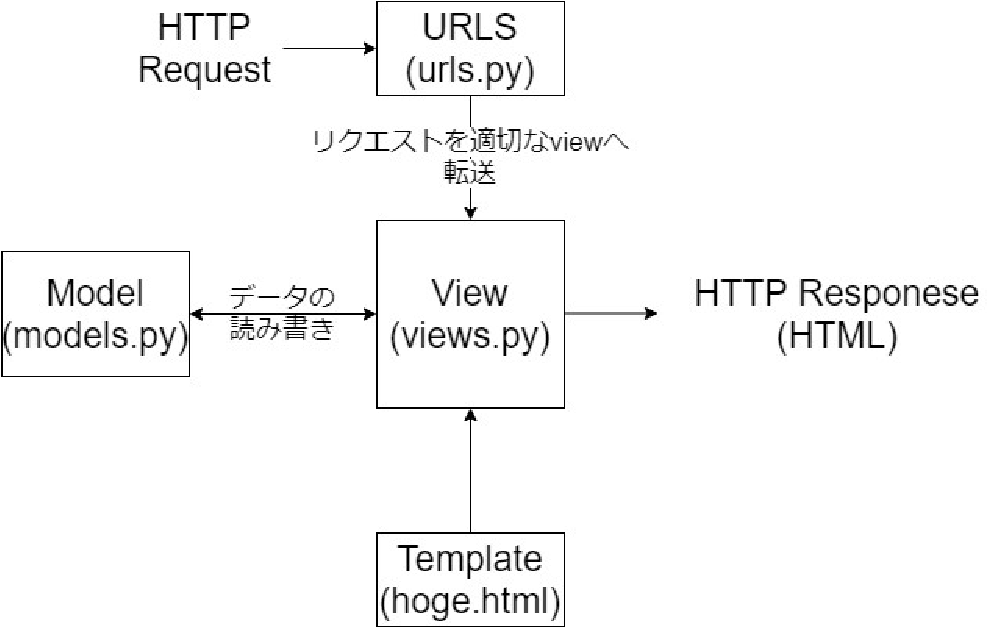
\includegraphics[width=13cm,height=12cm,keepaspectratio]{django_work-crop.pdf}\\
        %includegraphicsの詳しい使い方ははLaTeXの参考書を参照.
    \end{center}
    \caption{Djangoの動作の概要図}
    \label{django_work}
\end{figure}

URLSは単一URLから単一の関数を介してすべてのリクエストを処理することは可能だが,各リソースを処理する別々のView関数を作成する方がメンテナンスが容易なため,URLをマッピングしている.
これにより,URLに含まれる特定のパターンの文字列もしくは数字を照合し,これらをデータとしてView関数に渡して処理を行っている.

Viewは,HTTPリクエストを受け取り,HTTPレスポンスを返す関数である.
Viewはモデルを介して要求を満たすために必要なデータにアクセスし,レスポンスのフォーマットをTemplateに委任する.

Modelは,アプリケーションのデータ構造を定義し,データベース内のレコードを追加,変更,削除,および照会するための機能を提供するPythonオブジェクトである.

Templateは,ファイル構造やレイアウトを定義するテキストファイルで,プレースホルダを使用して実際のコンテンツを表示する.
Viewは,モデルから取得したデータとHTMLテンプレートを使用して動的にHTMLページを作成できる.
また,Templateを利用して,HTMLだけではなく,あらゆる種類のファイルの構造を定義できる.

\newpage
続いて,Djangoは複雑なデータベース主体のウェブサイトを簡単に構築するため,データベースを操作する3つの機能がある.
\begin{description}
    \item[・Djangoシェル]\mbox{}\\
        Djangoアプリケーションの環境を有効にしたままコマンドで操作が可能.
    \item[・マイグレーション]\mbox{}\\
        データベースの操作を一括に実行・取り消しを行うことが可能.
    \item[・管理サイト]\mbox{}\\
        Webブラウザで,データベースを操作することが可能. 
\end{description}
これらの機能を用いることにより,複雑なデータベース主体のウェブサイトを簡単に構築できる.

最後にDjangoで主に使用するコマンド一覧とその説明を表\ref{django_command}に示す.

\begin{table}[htb]
    \begin{center}
        \caption{Dockerコマンド一覧}
        \begin{tabularx}{\textwidth}{|l|X|}\hline
            manage.py createsuperuser & 管理者ユーザを作成する. \\ \hline
            manage.py changepassword & ユーザのパスワードを変更する. \\ \hline
            manage.py check & プロジェクトの構成チェック. \\ \hline
            manage.py dbshell & データベース管理用のシェルを起動する. \\ \hline
            manage.py dumpdata & データベースの内容をJson等の形式でエクスポートする. \\ \hline
            manage.py loaddata & データベースにdumpファイルをインポートする. \\ \hline
            manage.py makemigrations & マイグレーションファイルの作成. \\ \hline
            manage.py migrate & データベースにマイグレーションを摘葉する. \\ \hline
            manage.py shell & 管理者用のコマンドシェルを起動したいわモードに入る. \\ \hline
            manage.py startapp & 新規アプリケーションの作成. \\ \hline
            manage.py startproject & プロジェクトディレクトリの作成. \\ \hline
            manage.py test & テストフレームワークの実行. \\ \hline
            manage.py testserver & 検証用サーバを起動する. \\ \hline
            manage.py collectstatic & staticファイルの収集を行う. \\ \hline
            manage.py runserver & アプリケーションの起動を行う. \\ \hline
        \end{tabularx}
        \label{django_command}
    \end{center}
\end{table}

\subsubsection{Django REST framework}
Django REST framework\cite{drf}とはDjangoを使ってRESTfulなAPIを開発するために利用されるライブラリである.
Django REST frameworkを動作させるには,以下の要件を満たさなければならない.
\begin{enumerate}
    \item Python (3.5,3.6,3.7,3.8,3.9)
    \item Django (2.2,3.0,3.1)
\end{enumerate}


